
\section{Implementación}
En este capítulo expondremos la implementación tanto de la aplicación servidor como de la aplicación móvil.


\subsection{ Aplicación Servidor}
En capítulos anteriores ya comentamos la estructura de paquetes seguida para desarrollar el servidor, en este hablaremos de JPARepository.\\

JPARepository es un repositorio que nos ofrece métodos genéricos de gestión de clases persistentes como también métodos más concreto que nos permiten realizar operaciones complejas abstrayendonos de su implementacion.

Además este repositorio se adapta a la clase con la que va a trabajar.
\begin{lstlisting}[language=java,caption={Adaptación a la clase Usuario },label=DescriptiveLabel]
    
public interface UsuarioRepository 
extends JpaRepository<Usuario, Long> {
		}

\end{lstlisting} 
	



	
Como se puede ver en la figura \ref{jpa}, este interfaz importa la clase Usuario accediendo a todos sus atributos y generando una lista de métodos para estos atributos concretos como podemos ver en la siguiente.\\

\begin{lstlisting}[language=java,caption={Interfaz  de UsuarioRepository},label=jpa]
    
public interface UsuarioRepository 
extends JpaRepository<Usuario, Long> {

	public Usuario findByCorreo(String correo);

	public Usuario findByNombre(String nombre);

	public List<Usuario> findByNombreContaining
		(String nombre);

	@Override
	public <S extends Usuario> S save(S usuario);

	@Override
	public void delete(Long idUsuario);

	@Override
	public boolean exists(Long idUsuario);

	@Override
	public <S extends Usuario> S saveAndFlush(S usuario);

	@Override
	public Usuario findOne(Long idUsuario);
	}


\end{lstlisting} 









\subsubsection{API REST}




\begin{itemize}
\item \textbf{UsuarioController}


\begin{itemize}
\item \textbf{ /usuario/correo/\{correo\} [GET]}\\
Busca al usuario cuyo correo es el parámetro correo.

\begin{itemize}
\item Param 
\begin{itemize}
\item String correo
\end{itemize}
\item Reponse
\begin{itemize}
\item Usuario
\end{itemize}
\end{itemize}
\end{itemize}






\begin{itemize}
\item  \textbf{/usuario/nombre/\{nombre\} [GET]}\\
Busca al usuario cuyo nombre es el parámetro nombre.
\begin{itemize}
\item Param
\begin{itemize}
\item String nombre
\end{itemize}
\item Reponse
\begin{itemize}
\item Usuario
\end{itemize}
\end{itemize}
\end{itemize}


\begin{itemize}
\item \textbf{ /usuarios/lista/\{nombre\} [GET]}\\
Busca los usuarios que tienen el parámetro nombre como  parte de su nombre.

\begin{itemize}
\item Param
\begin{itemize}
\item String nombre
\end{itemize}

\item Reponse
\begin{itemize}
\item List<Usuario> 
\end{itemize}
\end{itemize}
\end{itemize}


\begin{itemize}
\item  \textbf{/usuario/ruta/\{idUsuario\} [GET]}\\
Busca las rutas cuyo propietario es el que tiene como identificador el idUsuario.
\begin{itemize}
\item Param
\begin{itemize}
\item  Long idUsuario
\end{itemize}
\item Reponse
\begin{itemize}
\item List<Ruta>
\end{itemize}
\end{itemize}
\end{itemize}
 


 \begin{itemize}
\item  \textbf{/usuario/pois/\{idUsuario\} [GET]}\\
Busca los pois cuyo propietario es el que tiene como identificador el idUsuario.
\begin{itemize}
\item Param
\begin{itemize}
\item Long idUsuario
\end{itemize}
\item Reponse
\begin{itemize}
\item List<Poi>
\end{itemize}
\end{itemize}
\end{itemize}


 \begin{itemize}
\item  \textbf{/usuario/pois/usuario/\{idUsuario\}/tipo [GET]}\\
Busca los pois cuyo propietario es el que tiene como identificador el idUsuario y por tipo de poi el tipo que le pasamos.
\begin{itemize}
\item Param
\begin{itemize}
\item Long idUsuario
\item String tipo
\end{itemize}
\item Reponse
\begin{itemize}
\item List(Poi)
\end{itemize}
\end{itemize}
\end{itemize}

\begin{itemize}
\item  \textbf{/usuario/ [POST]}\\
Crea un usuario.
\begin{itemize}

\item Body
\begin{itemize}
\item Usuario
\end{itemize}
\item Reponse
\begin{itemize}
\item Usuario
\end{itemize}
\end{itemize}
\end{itemize}

\begin{itemize}
\item  \textbf{/usuario/grupos/\{idUsuario\} [GET]}\\
Busca los grupos a los que pertenece el usuario con identificador idUsuario.
\begin{itemize}
\item Param
\begin{itemize}
\item Long idUsuario
\end{itemize}
\item Reponse
\begin{itemize}
\item List<Grupo>
\end{itemize}
\end{itemize}
\end{itemize}
 


\begin{itemize}
\item  \textbf{/usuario/\{idUsuario\} [DELETE]}\\
Elimina un usuario
\begin{itemize}
\item Param
\begin{itemize}
\item Long idUsuario
\end{itemize}
\end{itemize}
\end{itemize}


\begin{itemize}
\item  \textbf{/usuario/grupo/\{idGrupo\} [POST]}\\
Añade un usuario a un grupo.
\begin{itemize}
\item Param
\begin{itemize}
\item Long idGrupo
\end{itemize}
\item Body
\begin{itemize}
\item Usuario usuario
\end{itemize}

\end{itemize}
\end{itemize}
 

\begin{itemize}
\item  \textbf{/usuario/grupo/\{idGrupo\}/usuario/\{nombre\} [DELETE]}\\
Elimina a un usuario de un grupo.
\begin{itemize}
\item Param
\begin{itemize}
\item  Long idGrupo
\item String nombre
\end{itemize}
\end{itemize}
\end{itemize}



%%%%%%%%%%%%%%%%%%%%%%%%%%%%%%%%%%%%%%%%
% 
%%%%%%%%%%%%%%%%%%%%%%%%%%%%%%%%%%%%%%%%

\item \textbf{PoiController}
\begin{itemize}
\item  \textbf{/poi/ [POST]}\\
Crea un Poi.
\begin{itemize}
\item Body
\begin{itemize}
\item Poi
\end{itemize}
\item Reponse
\begin{itemize}
\item Poi
\end{itemize}
\end{itemize}
\end{itemize}

\begin{itemize}
\item  \textbf{/poi/\{idPoi\} [DELETE]}\\
Elimina un poi
\begin{itemize}
\item Param
\begin{itemize}
\item Long idPoi
\end{itemize}

\end{itemize}
\end{itemize}



%%%%%%%%%%%%%%%%%%%%%%%%%%%%%%%%%%%%%%%%
% 
%%%%%%%%%%%%%%%%%%%%%%%%%%%%%%%%%%%%%%%%
\item \textbf{GrupoController}
\begin{itemize}
\item  \textbf{/grupo/ [POST]}\\
Crea un grupo.
\begin{itemize}
\item Body
\begin{itemize}
\item Grupo
\end{itemize}
\end{itemize}
\end{itemize}


\begin{itemize}
\item \textbf{ /grupo/\{nombreGrupo\} [GET]}\\
Busca el grupo cuyo nombre es nombreGrupo.
\begin{itemize}
\item Param
\begin{itemize}
\item String nombreGrupo
\end{itemize}
\item Reponse
\begin{itemize}
\item Grupo
\end{itemize}
\end{itemize}
\end{itemize}





\begin{itemize}
\item  \textbf{/grupos/lista/\{nombreGrupo\} [GET]}\\
Devuelve una lista con los integrantes de un grupo cuyo nombre es nombreGrupo-
\begin{itemize}
\item Param
\begin{itemize}
\item String nombreGrupo
\end{itemize}
\item Reponse
\begin{itemize}
\item List<Usuario>
\end{itemize}
\end{itemize}
\end{itemize}
%%%%%%%%%%%%%%%%%%%%%%%%%%%%%%%%%%%%%%%%
% 
%%%%%%%%%%%%%%%%%%%%%%%%%%%%%%%%%%%%%%%%
\item \textbf{RutaController}

\begin{itemize}
\item  \textbf{/ruta/ [POST]}\\
Crea una ruta.
\begin{itemize}
\item Body
\begin{itemize}
\item Ruta
\end{itemize}
\item Reponse
\begin{itemize}
\item Ruta
\end{itemize}
\end{itemize}
\end{itemize}





\begin{itemize}
\item  \textbf{/rutacompartida/\{nombreGrupo\} [POST]}\\
Crea una ruta compartida para cada uno de los integrantes del grupo cuyo nombre es nombreGrupo.  Además envía una notificación push a cada integrante para indicar que la ruta ya esta disponible para comenzar.
\begin{itemize}
\item Param
\begin{itemize}
\item String nombreGrupo
\end{itemize}
\item Body
\begin{itemize}
\item Ruta 
\end{itemize}
\item Reponse
\begin{itemize}
\item Ruta
\end{itemize}
\end{itemize}
\end{itemize}


\begin{itemize}
\item \textbf{/rutacompartida/\{idRuta\} [GET]}\\
Busca todas las rutas cuyo parámetro idrutacompartida es idRuta.
\begin{itemize}
\item Param
\begin{itemize}
\item Long idRuta
\end{itemize}
\item Reponse
\begin{itemize}
\item List<Ruta>
\end{itemize}
\end{itemize}
\end{itemize}


\begin{itemize}
\item  \textbf{/rutaCompartida/\{idRuta\}/estado/\{estado\} [POST]}\\
Cambia el estado de la ruta cuyo identificador es idRuta.
\begin{itemize}
\item Param
\begin{itemize}
\item  Long idRuta
\item String estado
\end{itemize}
\item Reponse
\begin{itemize}
\item Ruta
\end{itemize}
\end{itemize}
\end{itemize}


\begin{itemize}
\item  \textbf{/rutacompartida/cerrar/\{idRuta\} [POST]}\\
Cierra la ruta cuyo identificador es idRuta. Y en el caso de que el resto de usuario ya hubieran cerrado sus rutas, elimina la invitación restante del usuario que queda.
\begin{itemize}
\item Param
\begin{itemize}
\item Long idRuta
\end{itemize}
\item Reponse
\begin{itemize}
\item Ruta
\end{itemize}
\end{itemize}
\end{itemize}


\begin{itemize}
\item  \textbf{/rutacompartida/seguimiento/ruta/\{idRuta\}/grupo/\{nombreGrupo\} [POST]}\\
Este servicio es el encargado de realizar el siguimiento de los usuario. Envía una lista con los punto seguidos durante la ruta cuyo identificador es idRuta del usuario y además recibe una lista con los últimos puntos de cada uno de los integrantes del grupo cuyo nombre es nombreGrupo.
\begin{itemize}
\item Param
\begin{itemize}
\item String nombreGrupo
\item Long idRuta
\end{itemize}
\item Body
\begin{itemize}
\item List<PuntoRuta> puntosRutaEntrada
\end{itemize}
\item Reponse
\begin{itemize}
\item List<PuntoRuta>
\end{itemize}
\end{itemize}
\end{itemize}


\begin{itemize}
\item  \textbf{/ruta/\{idRuta\} [DELETE]}\\
Elimina la ruta con identificador idRuta.
\begin{itemize}
\item Param
\begin{itemize}
\item Long idRuta
\end{itemize}
\end{itemize}
\end{itemize}



\begin{itemize}
\item  \textbf{/ruta/puntos/\{idRuta\} [GET]}\\
Obtiene todos los puntos de la ruta que tiene como identificador el idRuta.
\begin{itemize}
\item Param
\begin{itemize}
\item Long idRuta
\end{itemize}
\item Reponse
\begin{itemize}
\item List<PuntoRuta>
\end{itemize}
\end{itemize}
\end{itemize}






\begin{itemize}
\item  \textbf{/ruta/lista/\{idRuta\} [GET]}\\
Obtiene una lista con rutas que fueron compartidas a la vez que la ruta cuyo idRutaCompartida es idRuta.
\begin{itemize}
\item Param
\begin{itemize}
\item Long idRuta
\end{itemize}
\item Reponse
\begin{itemize}
\item List(Ruta)
\end{itemize}
\end{itemize}
\end{itemize}




%%%%%%%%%%%%%%%%%%%%%%%%%%%%%%%%%%%%%%%%
% 
%%%%%%%%%%%%%%%%%%%%%%%%%%%%%%%%%%%%%%%%
\item \textbf{PuntoRutaController}


\begin{itemize}
\item \textbf{ /puntoruta/\{idRuta\} [POST]}\\
Guarda una lista de puntos asociados a una ruta que tiene como identificador idRuta.
\begin{itemize}
\item Param
\begin{itemize}
\item Long idRuta
\end{itemize}
\item Body
\begin{itemize}
\item List<PuntoRuta> puntosRutaEntrada
\end{itemize}
\item Reponse
\begin{itemize}
\item List<PuntoRuta>
\end{itemize}
\end{itemize}
\end{itemize}
\end{itemize}

En la anterior API se usan una serie de objetos que hacen referencia a las siguientes interfaces:
\begin{itemize}
 \item Usuario ver figura \ref{fig:Usuario}
 \item Grupo ver figura \ref{fig:Grupo}
 \item Ruta ver figura \ref{fig:Ruta}
 \item PuntoRuta ver figura \ref{fig:PuntoRuta}
 \item Poi ver figura \ref{fig:Poi}
\end{itemize}





































\begin{figure}[H]
\begin{minipage}[b]{0.5\linewidth}
\centering
\begin{tikzpicture} 
\umlinterface{Usuario}
{Long idusuario 
\\ String nombre
\\ String correo
\\ String password
\\ String token}{} 
\end{tikzpicture}
\caption{ Interfaz Usuario}
\label{fig:Usuario}
\end{minipage}
\begin{minipage}[b]{0.5\linewidth}
\centering
\begin{tikzpicture} 
\umlinterface{Grupo}
{Long idGrupo 
\\ String nombre 
}{} 
\end{tikzpicture}
\caption{ Interfaz Grupo}
\label{fig:Grupo}
\end{minipage}
\end{figure}




\begin{figure}[H]
\begin{minipage}[b]{0.5\linewidth}
\centering
\begin{tikzpicture} 
\umlinterface{Ruta}
{Long idRuta 
\\ String nombre 
\\ String estado 
\\ Long idrutacompartida}{} 
\end{tikzpicture}
\caption{ Interfaz Ruta}
\label{fig:Ruta}
\end{minipage}
\begin{minipage}[b]{0.5\linewidth}
\centering
\begin{tikzpicture} 
\umlinterface{PuntoRuta}
{Long idpuntoruta 
\\ Double latitud 
\\ Double longitud 
\\ number: string}{} 
\end{tikzpicture}
\caption{ Interfaz PuntoRuta}
\label{fig:PuntoRuta}
\end{minipage}
\end{figure}




\begin{figure}[H]
\begin{minipage}[b]{0.5\linewidth}
\centering
\begin{tikzpicture} 
\umlinterface{Poi}
{Long idpoi 
\\ String nombre 
\\ String tipo 
\\ Double latitud
\\ Double longitud
\\String descripcion}{} 
\end{tikzpicture}
\caption{ Interfaz Poi}
\label{fig:Poi}
\end{minipage}
\end{figure}














\newpage

 
 
 
 
 \subsection{Aplicación móvil Android}
En este capítulo comentaremos aspectos concretos de la implementación de de la aplicación móvil \cite{8}.



\subsubsection{Mapas}

 Para la creación de rutas tanto individuales como compartidas como para crear PDI el usuario necesita conocer las coordenadas de los puntos por lo que transcurre su ruta. Para ello necesitamos los mapas de Google Maps y métodos de sus APIs.
 
 
 \begin{lstlisting}[language=java,caption={Dependencia de Google Maps en gradle},label=map]
compile 'com.google.android.gms:play-services-maps:10.2.0'

\end{lstlisting}
 
 Con la dependencia de la figura \ref{map} permitimos a nuestra aplicación que use los servicios de  Google Maps.\\
 Para marcar un punto en el mapa y que este quede visible en este necesitamos implementar un método que capture los clic en el mapa y que nos devuelva las coordenadas del punto marcado.
 
 
 \begin{lstlisting}[language=java,caption={Captura de clic en la pantalla},label=clic]
    
mMap.setMyLocationEnabled(true);
mMap.getUiSettings().setCompassEnabled(true);
mMap.setOnMapClickListener(new GoogleMap
	.OnMapClickListener() {
	public void onMapClick(LatLng point) {
	mMap.clear();
	poilongitud = point.longitude;
	poilatitud = point.latitude;
	LatLng Yo = new LatLng(poilatitud, poilongitud);
	Marker mensaje = 
	mMap.addMarker(new MarkerOptions()
		.position(Yo)
		.title("Guardar este punto?"));
  	mensaje.showInfoWindow();
	VerTodosPois();

\end{lstlisting} 
 
 
 
 
  Con el fragmento de código de la figura \ref{clic}  se capturaría ese clic y aparecería el Marker común de todos los mapas de Google Maps acompañado del mensaje \textit{"Guardar este punto?"}. En nuestro proyecto personalizamos los Marker de modo que cuando guardamos ese punto pase a a representarse con icono de un pescador o de un cazador dependiendo del PDI que estuviéramos guardando. Para ello usamos el siguiente fragmento de código.

 

\begin{lstlisting}[language=java,caption={Creación de Marker  personalizados},label=DescriptiveLabel]
    
protected Marker createMarkerPesca(double
		latitude,Double longitude, String nombre,
		String	descripcion) {
       		return mMap.addMarker(new MarkerOptions()
                	.position(new LatLng(latitude, 							longitude))
                	.anchor(0.5f, 0.5f)
                	.title(nombre).snippet(descripcion)
	                .icon(BitmapDescriptorFactory
    	       		.fromResource(R.drawable.pescador)));
    }


\end{lstlisting} 
 
 
 
 Y así es como quedaría en la figura~\ref{fig:marker5} y figura \ref{fig:marker6}

 
 
 
	\begin{figure}
\begin{minipage}[b]{0.5\linewidth} %Una minipágina que cubre la mitad de la página
\centering
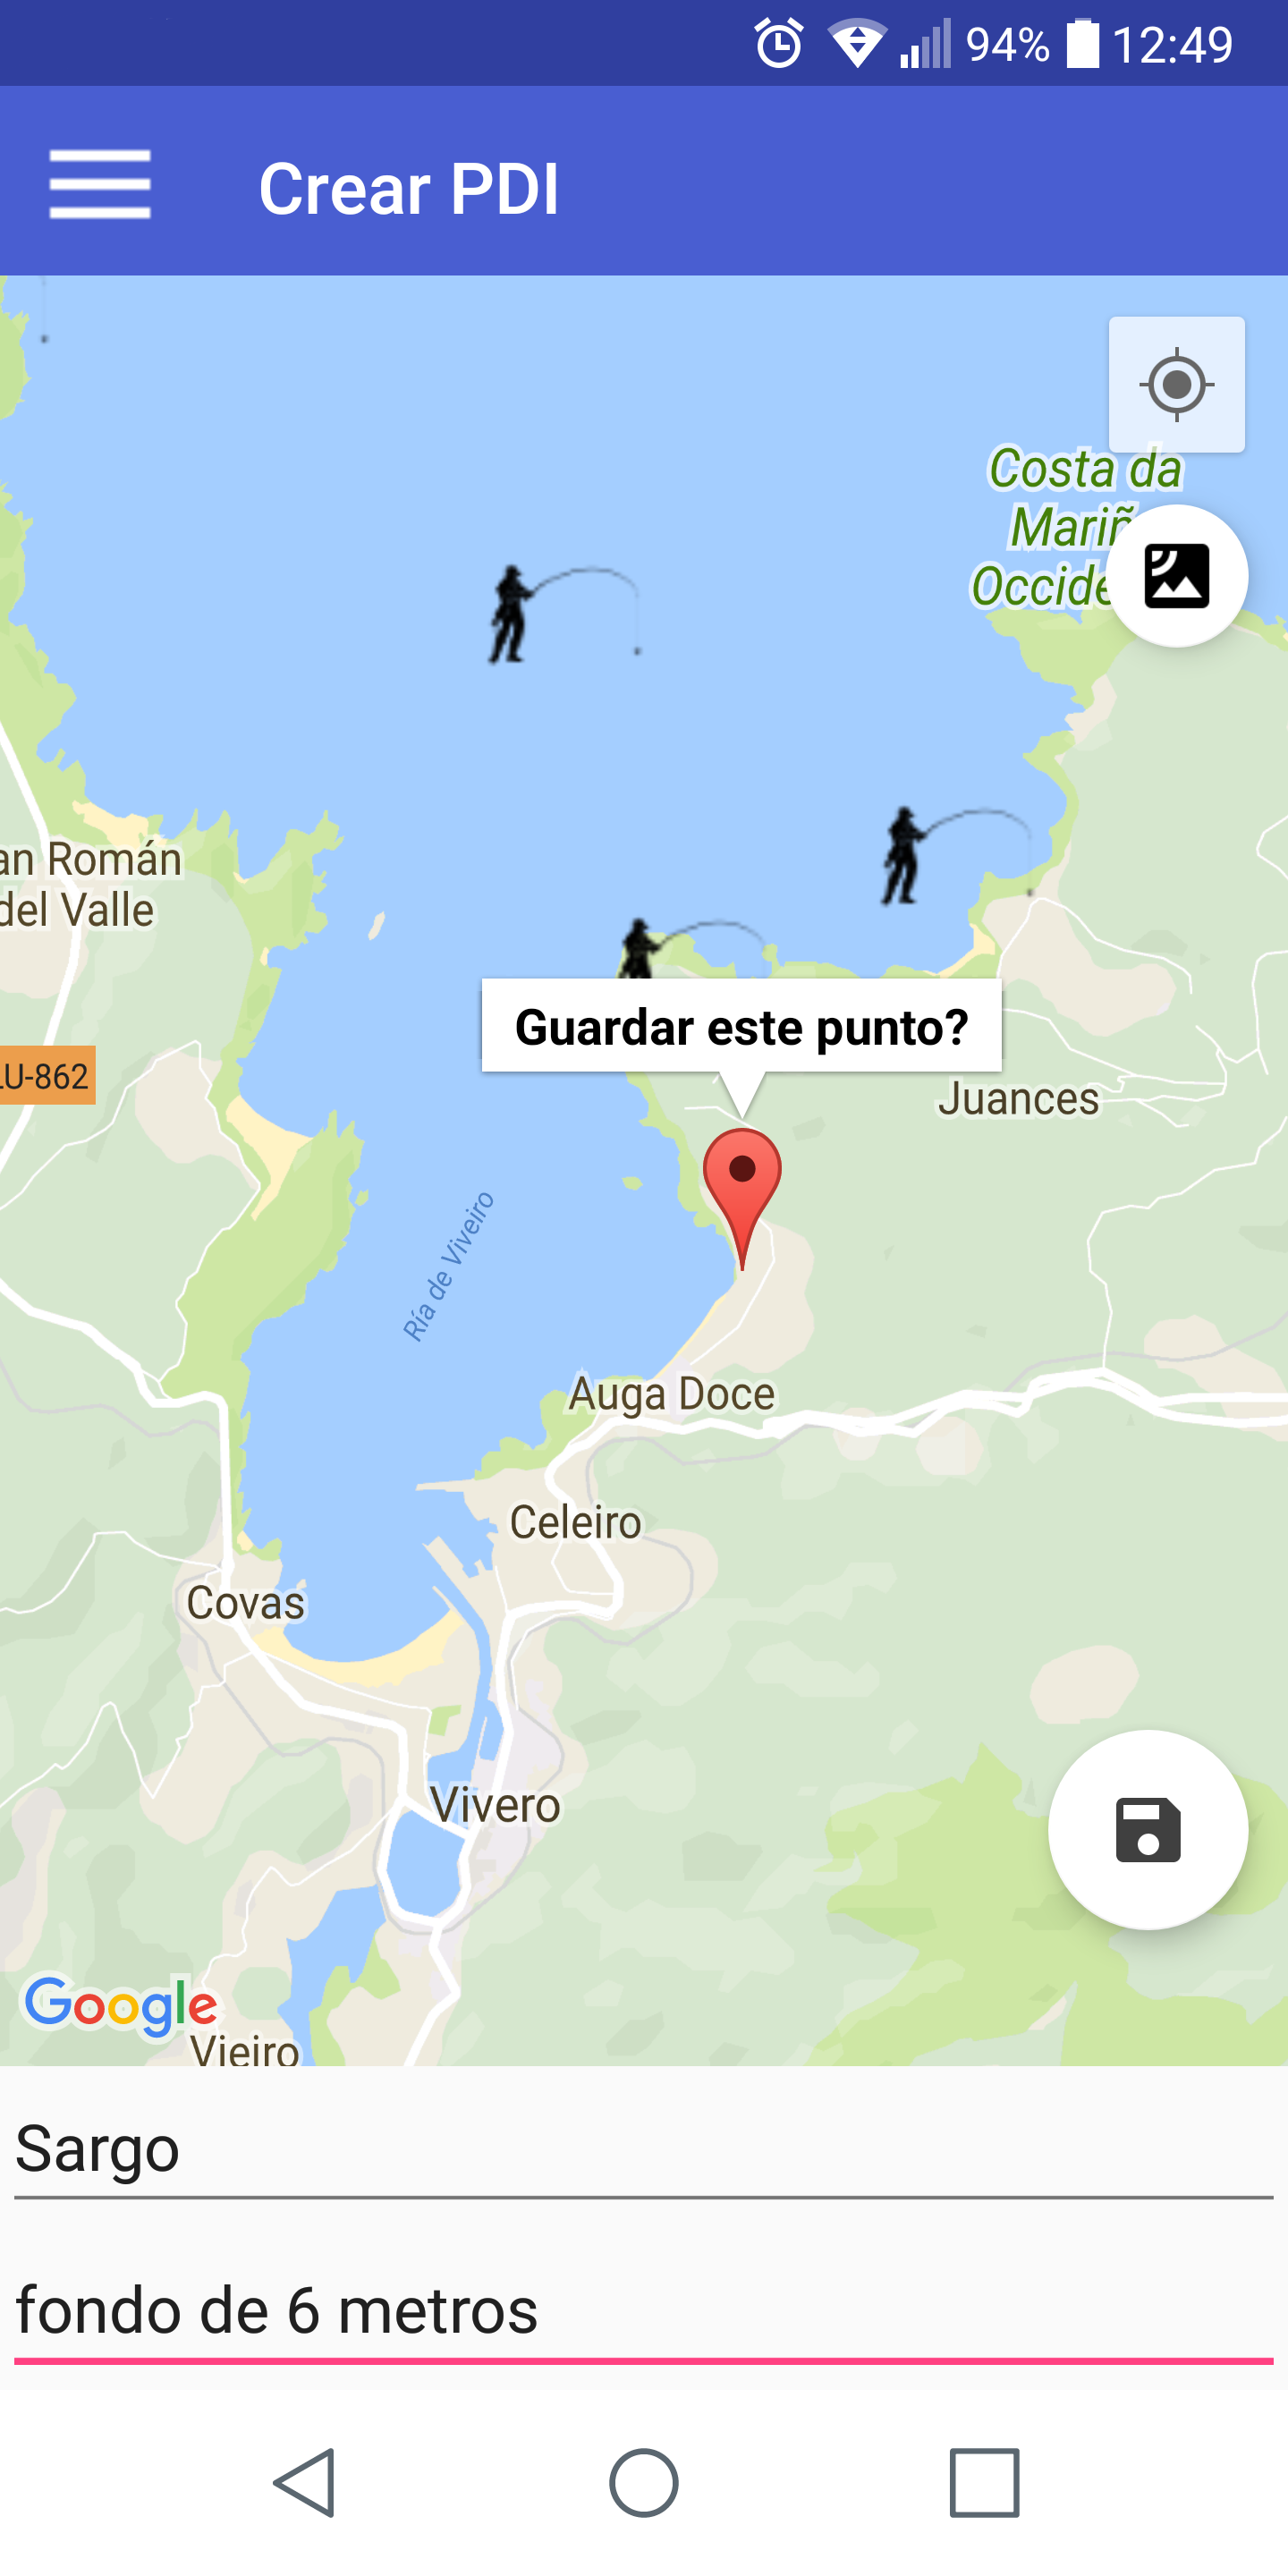
\includegraphics[width=6cm]{capturamovil/pdiguardar.png}
 \label{marker5}
\caption{Marker antes de guardar el PDI}

\end{minipage}
\hspace{0.5cm} % Si queremos tener un poco de espacio entre las dos figuras
\begin{minipage}[b]{0.5\linewidth}
\centering
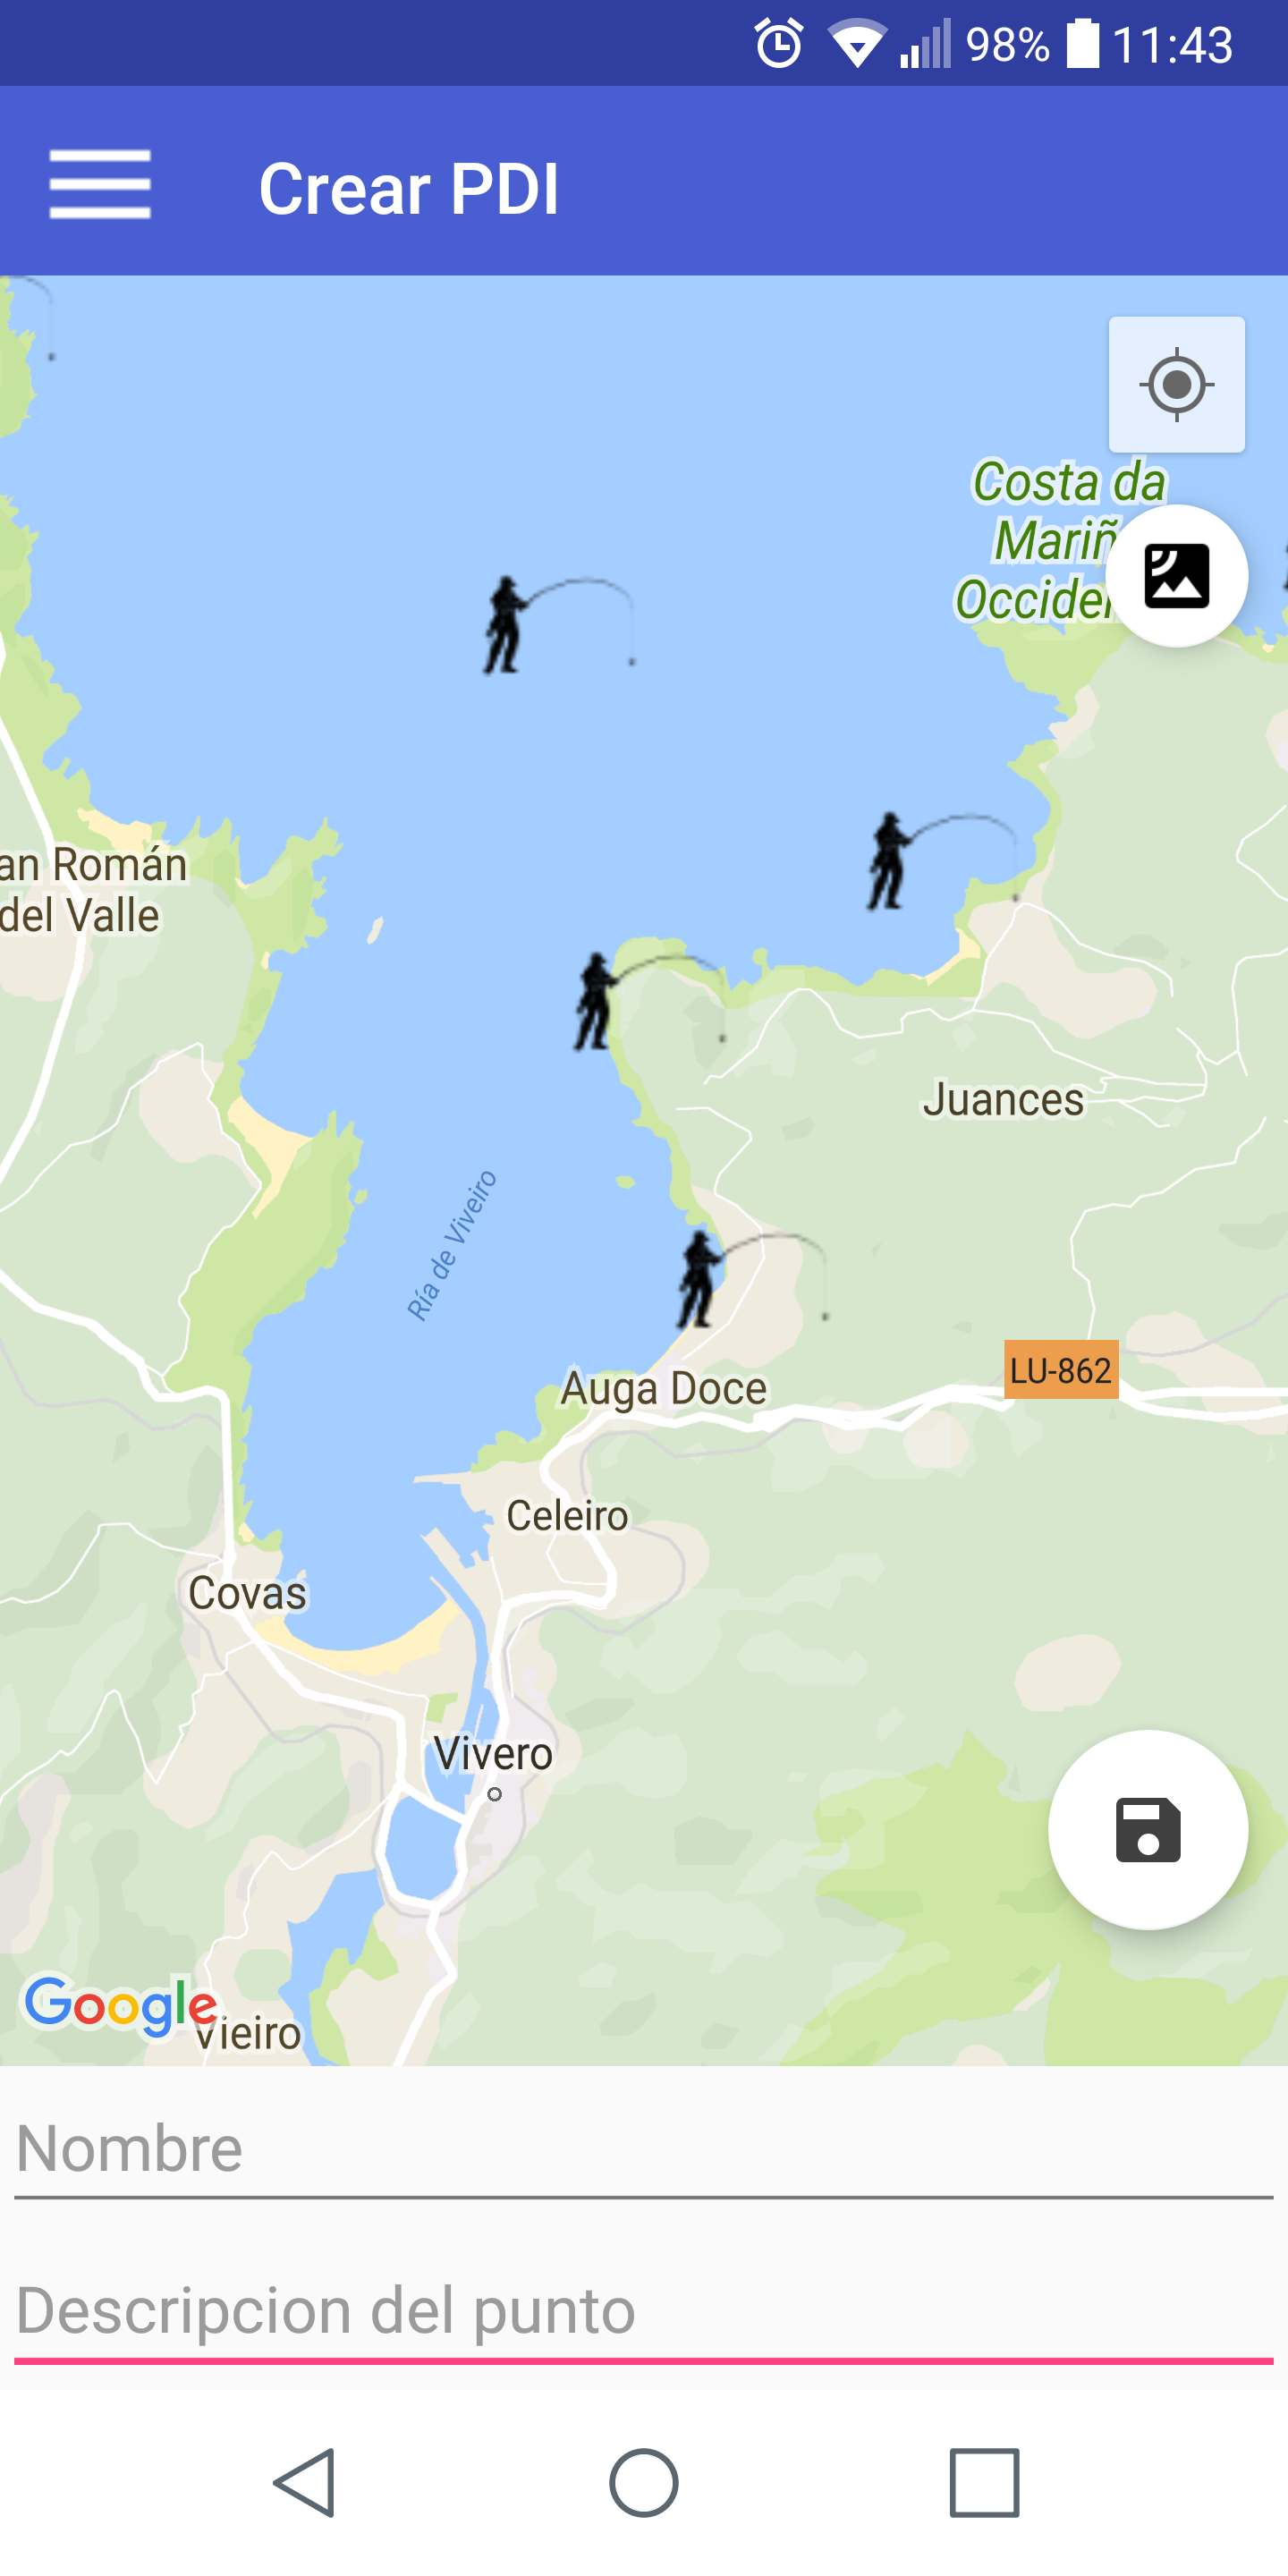
\includegraphics[width=6cm]{capturamovil/pdiguardar2.png}
 \label{marker6}
\caption{Marker después }

\end{minipage}
		\label{fig:marker}

\end{figure} 
 
 
 
 \subsubsection{Localización}
  Para la creación de ruta necesitamos un método que nos proporcione las coordenadas(latitud y longitud) de los puntos por los que transcurre el usuario en la ruta. Para ellos necesitamos la siguiente dependencia.

	
\begin{lstlisting}[language=java,caption={Dependencia de Location en gradle},label=DescriptiveLabel]
compile 'com.google.android.gms:play-services-location:10.2.0'


\end{lstlisting}	
	
	
	Una vez añadida esta dependencia necesitamos un método que nos proporciones las coordenadas concretas, para ellos usaremos el siguiente fragmento de código.
	
\begin{lstlisting}[language=java,caption={Obtencion de coordenadas  por intervalo de tiempo},label=distancia]
mlocManager.requestLocationUpdates(LocationManager
.GPS_PROVIDER  15   , 0,(LocationListener) Local);


\end{lstlisting}	

El método ofrece el par de coordenadas cuando el usuario se mueve 15 metros o bien por un intervalo de tiempo en segundos.


Como se puede observar en la figura \ref{distancia} en nuestro proyecto indicamos que los segundos que deberían transcurrir para devolver unas coordenadas sería de 15.\\
Cuando nosotros estamos realizando la ruta en ocasiones el GPS pierde precisión y sitúa al usuario en punto un tanto lejano, lo cual es imposible ya que no se puede mover tan rápido. Este error del GPS lo hemos resuelto de la siguiente manera, el código \ref{variacion} .\\




\begin{lstlisting}[language=java,caption={Fragmento para el calculo de distancias entre puntos},label=variacion]
      iniTramo = finTramo;
      finTramo = new LatLng(latitud, longitud);
      Location location1 = new Location("localizacion 1");
      location1.setLatitude(iniTramo.latitude);  //latitud
      location1.setLongitude(iniTramo.longitude); //longitud
      Location location2 = new Location("localizacion 2");
      location2.setLatitude(finTramo.latitude);  //latitud
      location2.setLongitude(finTramo.longitude); //longitud
      double distance = location1.distanceTo(location2);
\end{lstlisting}

En este código lo que hacemos es calcular la distancia entre dos puntos consecutivos. Usamos un método que pertenece a la API,  el cual necesita un par de coordenadas. El dato que devuelve viene dado en metros y  dado tiene en cuenta la curvatura de la tierra para calcularlo. Si esta distancia es superior a 15 metros desechamos ese punto. El resultado de los puntos válidos lo podemos ver en  Figura~\ref{fig:individual-navegacion2}

\begin{figure}
		\centering
		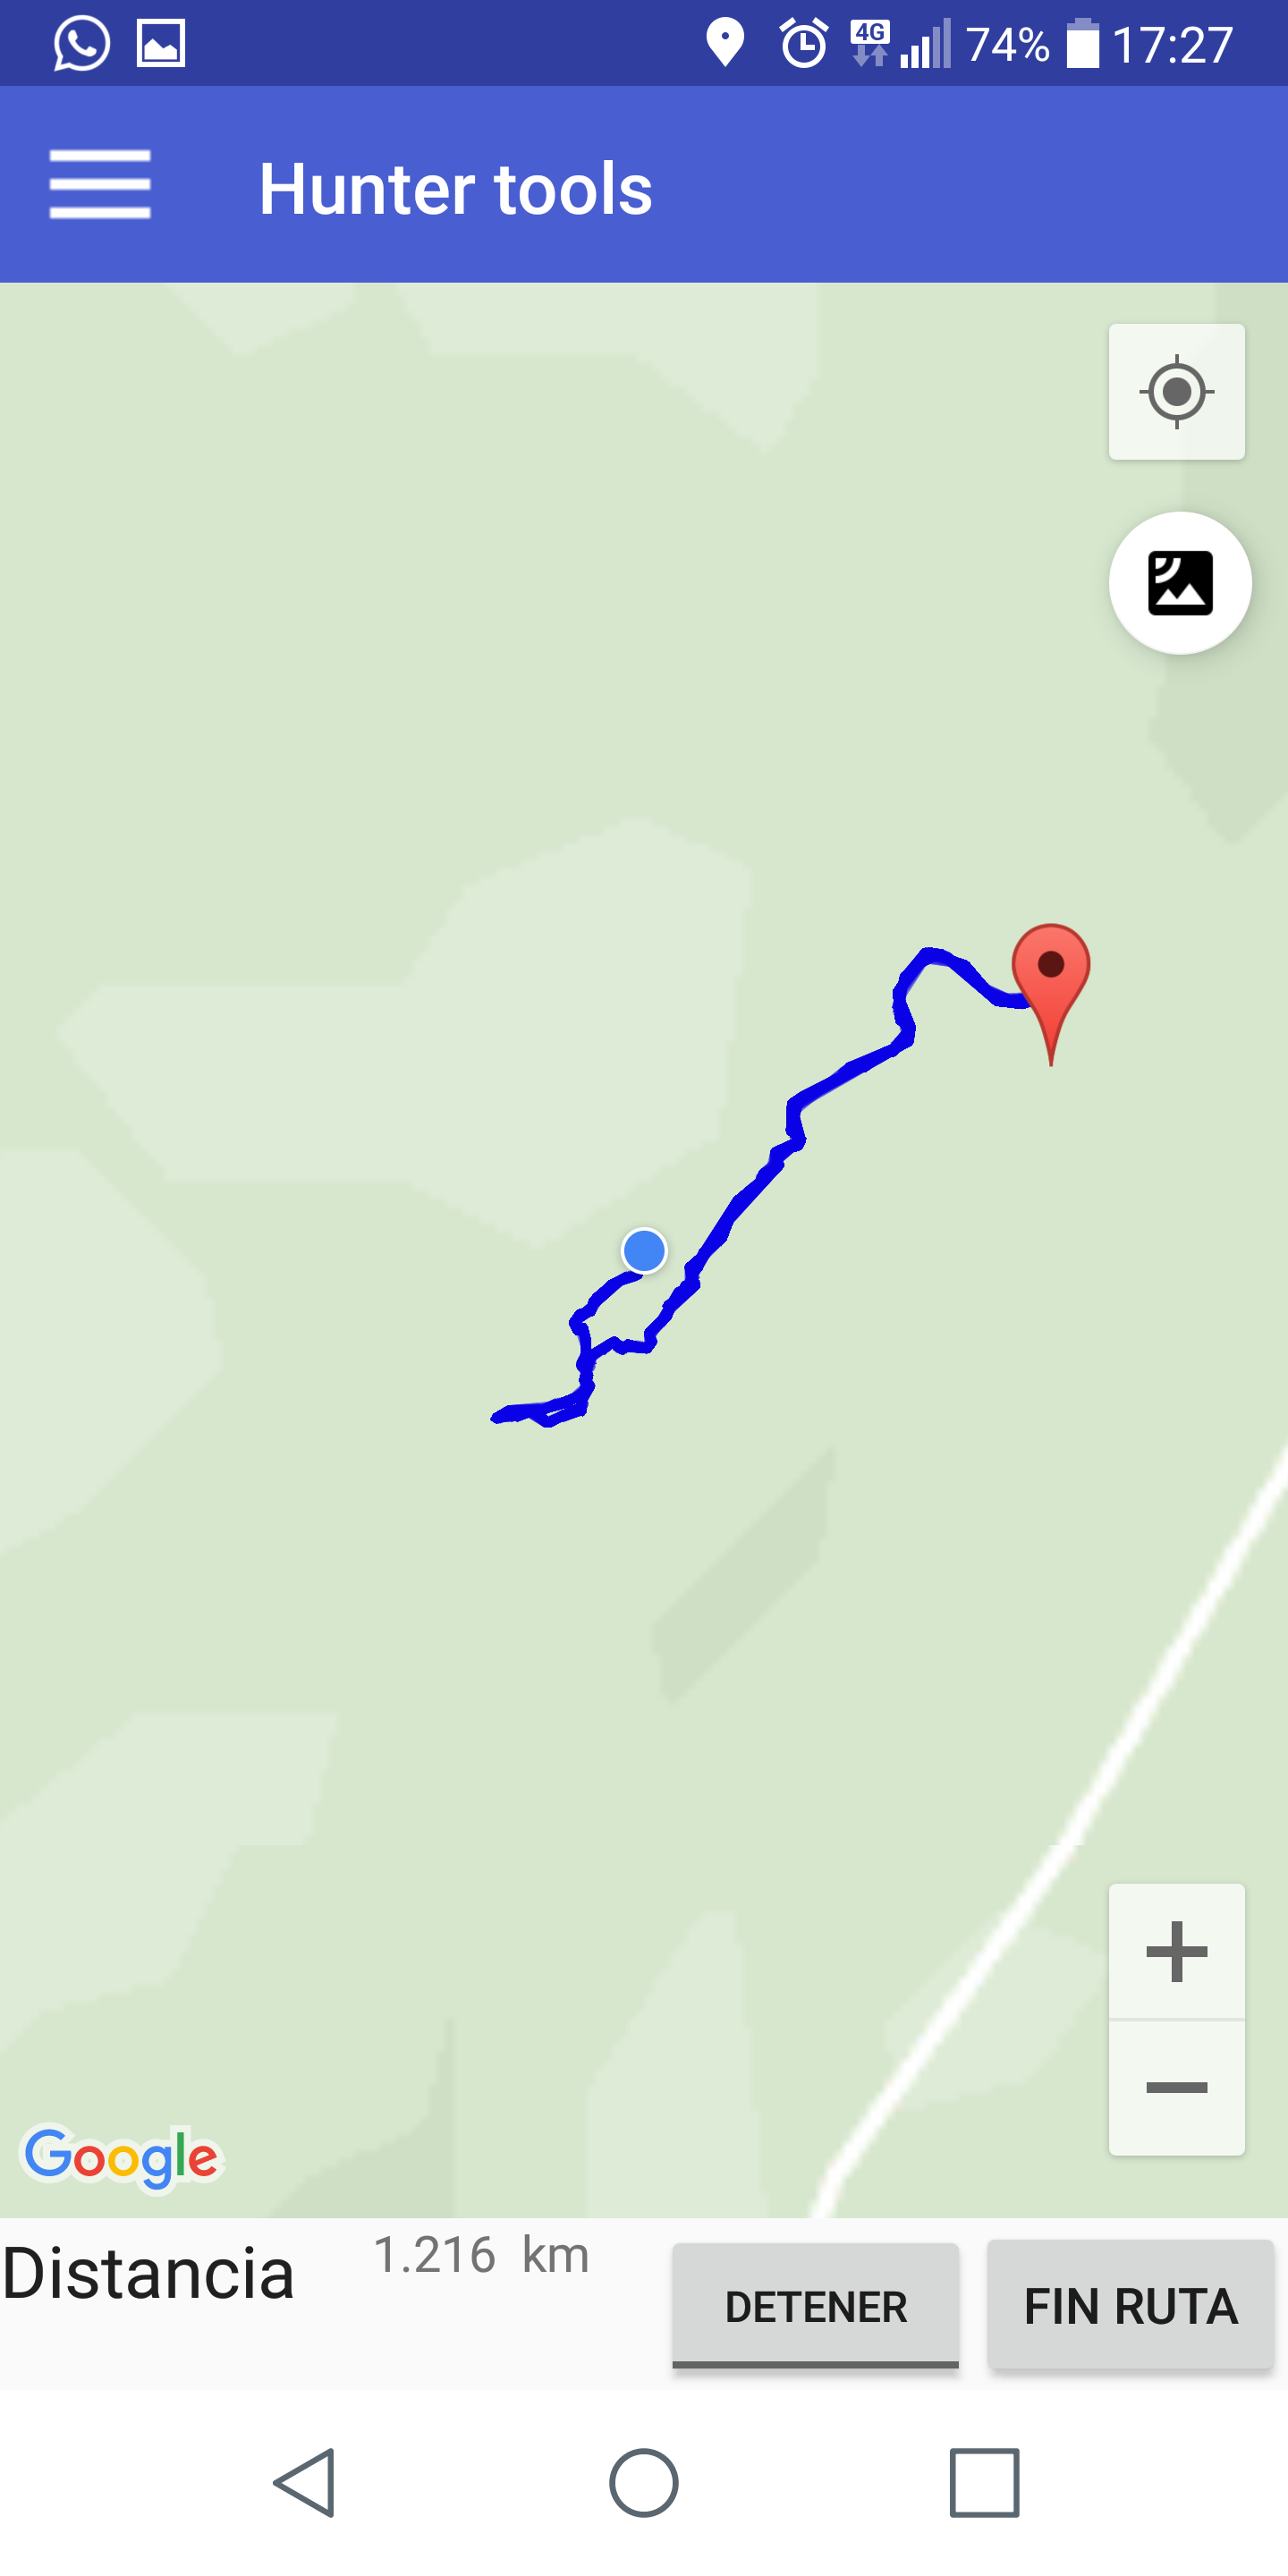
\includegraphics[width=0.4\textwidth] {capturamovil/individual-navegacion.png}
		\caption{Visualización de la ruta mientras se realiza}
		\label{fig:individual-navegacion2}
	\end{figure}
	
\subsubsection{Firebase} 
Cuando el usuario inicia una ruta compartida el sistema avisa al resto de integrantes de grupo de que acaban de ser invitados a ella, esta acción la realizamos mediante las Notificaciones Push con Firebase \cite{7}. Para ello tenemos que empezar añadiendo las dependencias siguientes.

	\begin{lstlisting}[language=java,caption={Dependencia de Firebase en gradle},label=DescriptiveLabel]
 compile 'com.google.firebase:firebase-core:10.2.0'
 compile 'com.google.firebase:firebase-messaging:10.2.0'

\end{lstlisting}
	
Del lado del servidor enviamos una notificación con una serie de campos necesarios para identificar la ruta a un usuario concreto. Este usuario lo identificamos por un token que almacenamos en la base de datos, este token es característico de cada móvil. Para que nuestra aplicación  pueda recibir y entender esta notificación necesitaremos el siguiente fragmento de código.
	\begin{lstlisting}[language=java,caption={Recepción de mensajes},label=DescriptiveLabel]
 @Override
 public void onMessageReceived(RemoteMessage remoteMessage) {
        Map<String, String> data = remoteMessage.getData();
        titulo= data.get("titulo");
        nombreGrupo= data.get("nombreGrupo");
        accion= data.get("accion");
        idRuta= data.get("idRuta");
        verAccionString ();
        EventBus.getDefault().post(remoteMessage
        .getData().toString());
      
           }
\end{lstlisting}
Este método pasearía el JSON que envía el servidor y guardaría los datos necesario en el móvil.
En la siguiente captura veríamos la notificación en el móvil.	
	
	\begin{figure}[htbp]
\begin{minipage}[b]{0.5\linewidth} %Una minipágina que cubre la mitad de la página
\centering
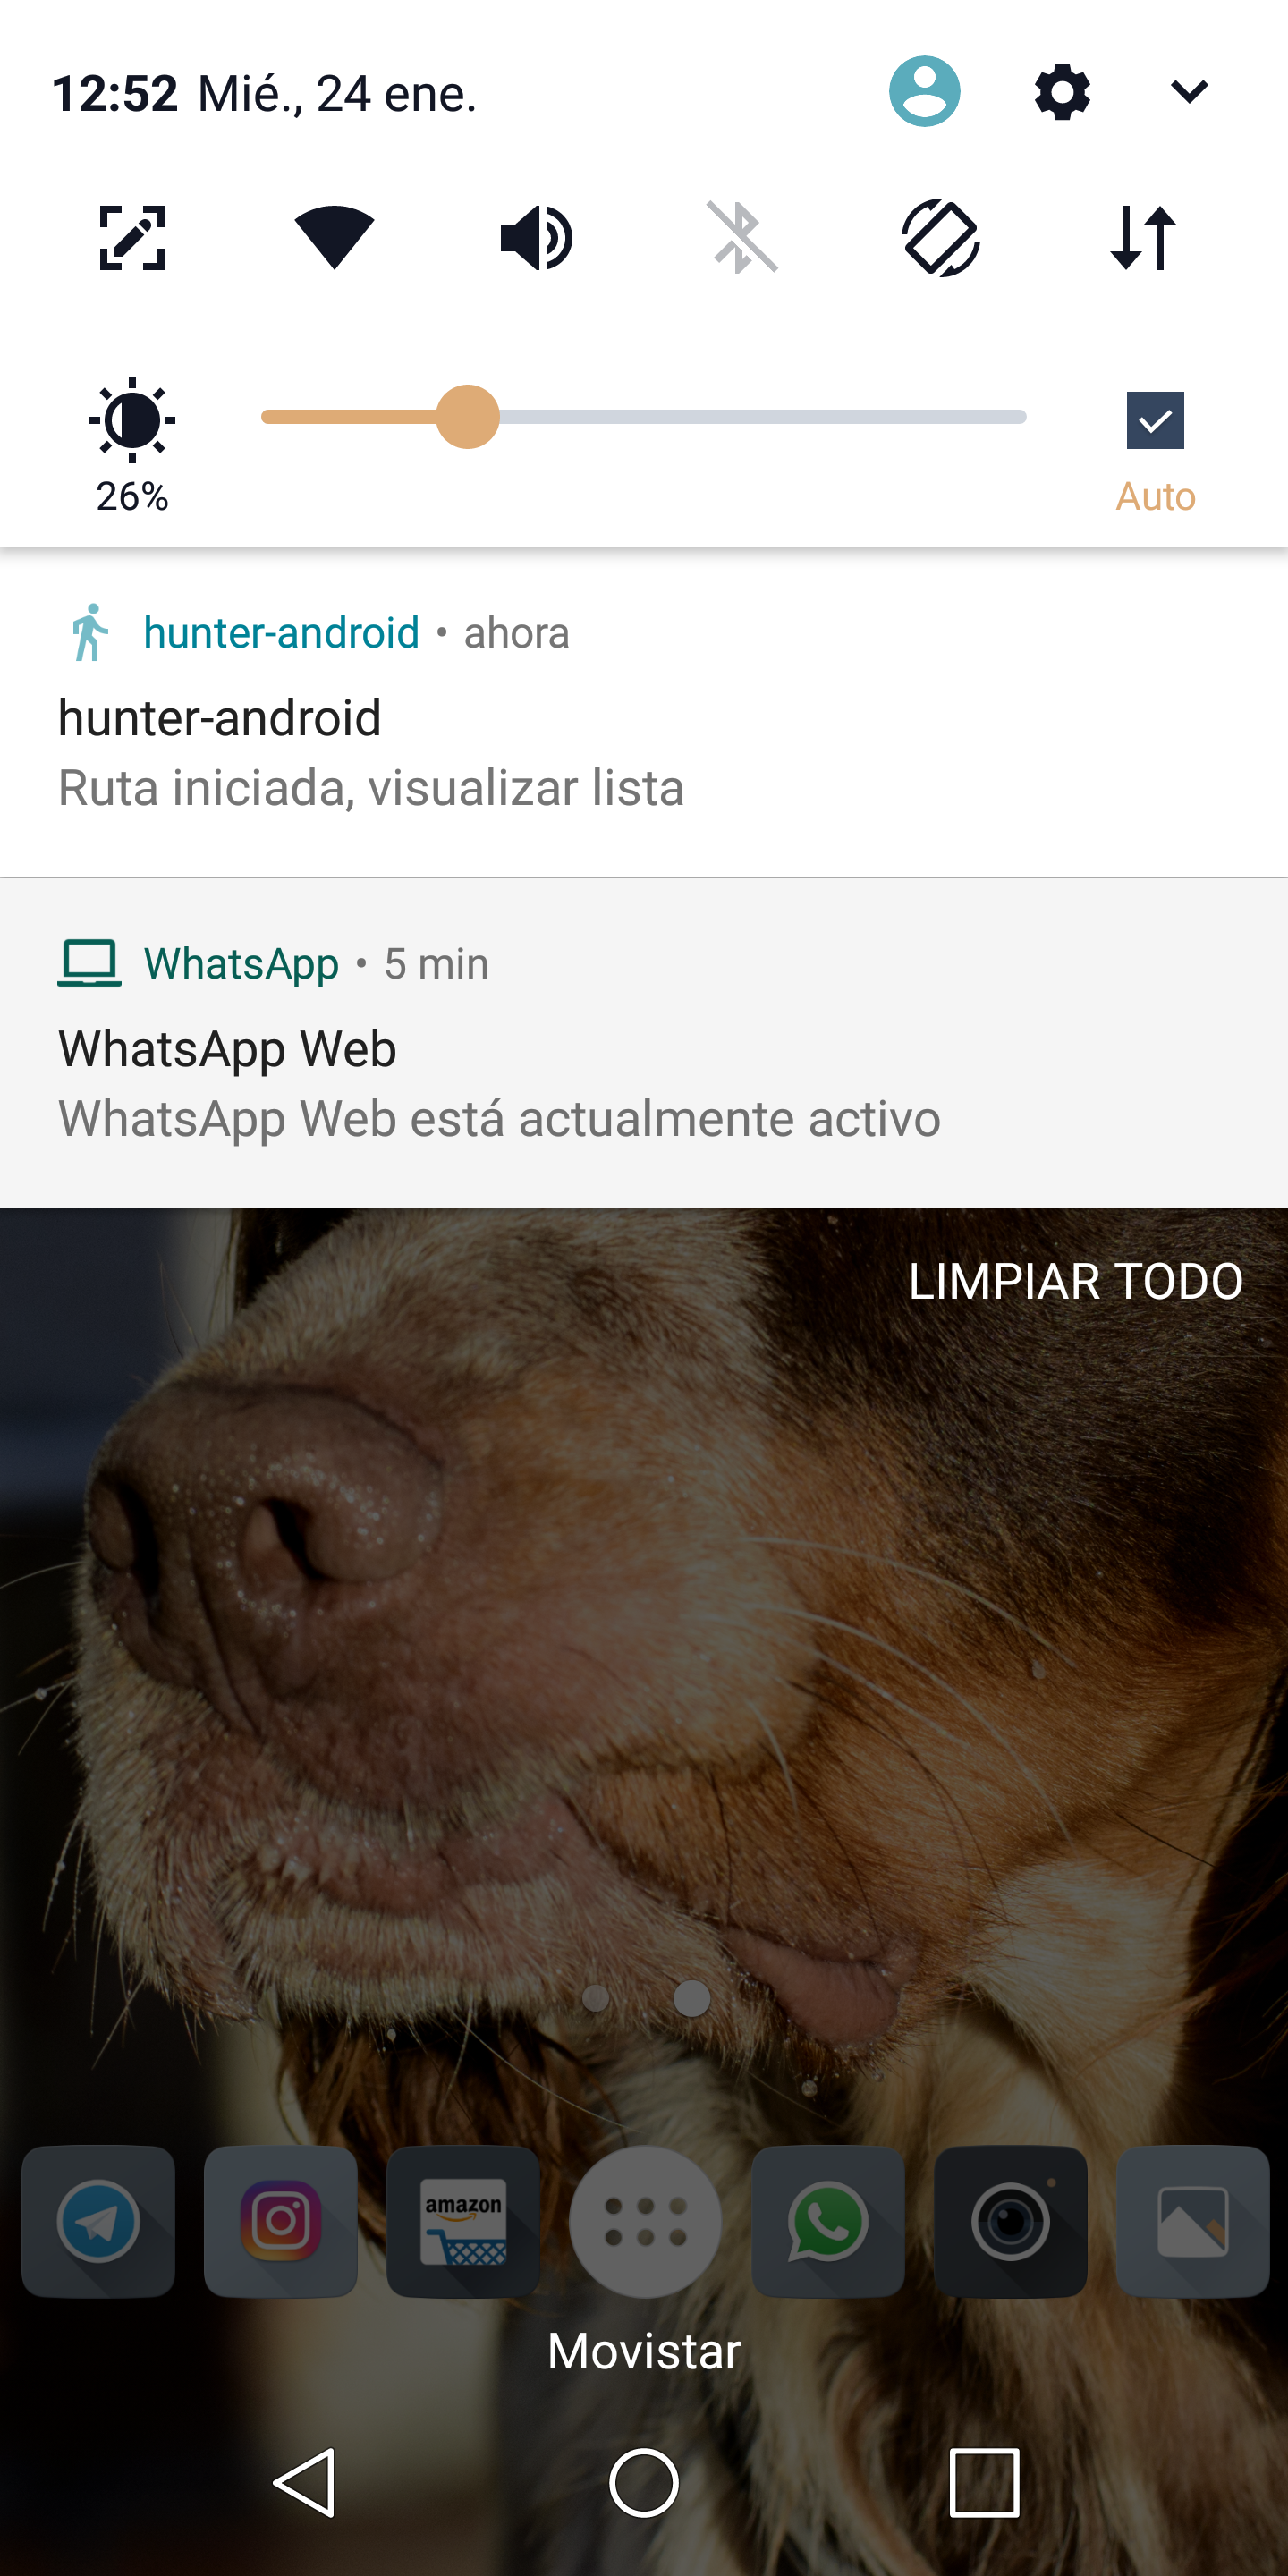
\includegraphics[width=6cm]{capturamovil/push1.png}
 \label{figura1}

\end{minipage}
\hspace{0.5cm} % Si queremos tener un poco de espacio entre las dos figuras
\begin{minipage}[b]{0.5\linewidth}
\centering
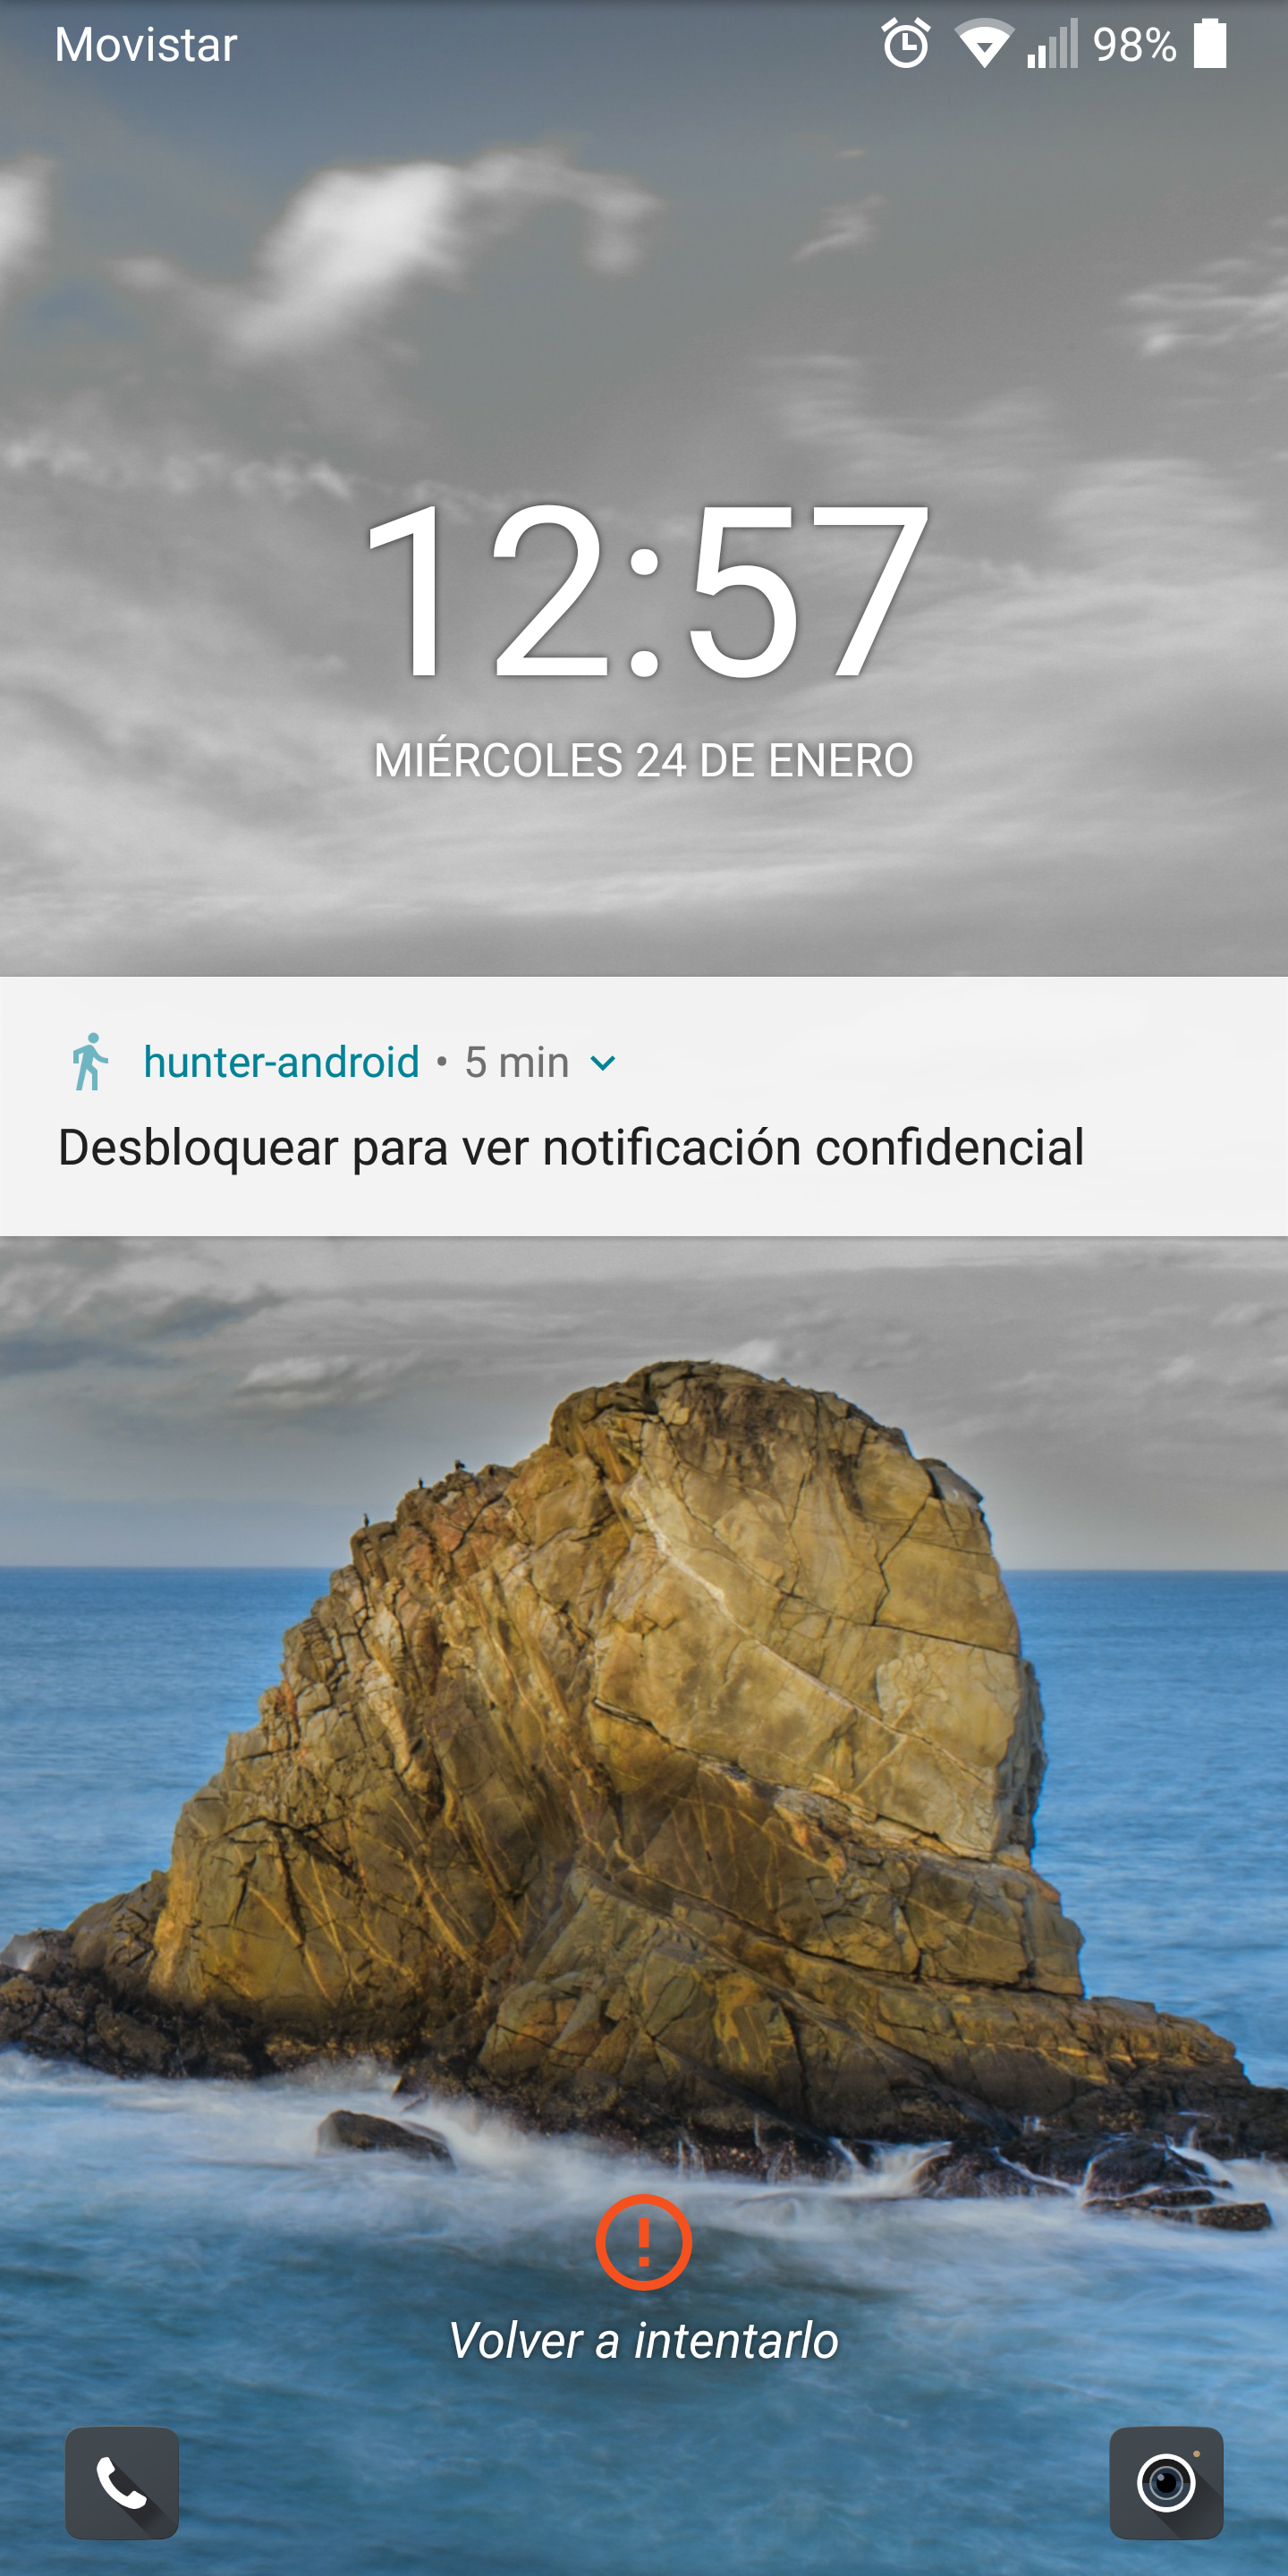
\includegraphics[width=6cm]{capturamovil/push2.png}
 \label{figura2}

\end{minipage}
\caption{Notificación push }
\end{figure} 
 
	
\newpage
	
\section{Pruebas}
Las pruebas son un tema muy importante a tener en cuenta en cualquier proyecto de software. Nos permiten conocer ciertos aspectos que fallan en el sistema de manera objetiva y conocer ciertos riesgos que se nos pasaron por alto en la implementación.
Dado que usamos la metodología Scrum y como describimos en el capítulo de seguimiento al final de cada Sprint se harán las pruebas para esas historias de usuario.



\subsection{Pruebas de unidad}
Las pruebas de unidad se  encargan de comprobar el  buen funcionamiento de partes de código. Esta comprobación se realiza normalmente a nivel de clase  asegurándonos que el funcionamiento es el adecuado.\\En nuestro caso las pruebas de unidad se realizaron en el servidor ayudándonos del framework de pruebas JUnit. Como ya se comentó JUnit es una tecnología que ayuda a la ejecución de pruebas  para la comprobación del funcionamiento de métodos o clases.

Como también se usó el framework Spring para el desarrollo este también fue empleado para los test ya que ayuda a la inyección de dependencias y otras gestiones de las transacciones.



\begin{lstlisting}[language=java,
 ,backgroundcolor=\color{backcolour},   
    commentstyle=\color{codegreen},
    keywordstyle=\color{magenta},
    numberstyle=\tiny\color{codegray},
    stringstyle=\color{codepurple}]
@RunWith(SpringJUnit4ClassRunner.class)
@WebAppConfiguration
@Profile("test")
@ContextConfiguration("classpath:root-context.xml")
public class UsuarioServiceTest {

	@Autowired
	private UsuarioService usuarioService;
	
	@Test
	public void testPruebaUsuario() {
	Usuario u1 = new Usuario("tito", "titef@udc.es", "pass");
		u1 = usuarioService.save(u1);
		Usuario u2;
		u2 = usuarioService.findByCorreo("titef@udc.es");
		(u2.getNombre()).equals("tito");
		usuarioService.delete(u1.getIdusuario());
}
\end{lstlisting}







\subsection{Pruebas de integración y aceptación}
Las pruebas de integración entre los componentes del sistema y las de aceptación se realizaron de forma manual. En ellas se comprobaba el funcionamiento y la respuesta antes las acciones realizadas.\\
Como el servidor estaba desplegado en un servidor de aplicaciones las pruebas se podían realizar de 2 maneras:
\begin{itemize}
\item Mediante el emulador propio de Android.\\
Esta opción fue la utilizada para depurar la aplicación en los primeros Sprint ya que era más cómodo a la hora realizar las pruebas usar el teclado.
\item  Mediante un móvil en el cual se instalaba nuestra aplicación. En cambio esta opción  fue la más utilizada en los últimos sprints ya que requerían unas pruebas más reales en  lugares abiertos, ya que se perseguía la comprobación de la precisión del GPS  en casos reales de uso. Esto fue clave para mejora de la creación de rutas.
\end{itemize}







